\documentclass[english, DIV=13]{scrartcl}

% Packages
\usepackage[utf8x]{inputenc}
\usepackage[T1]{fontenc}
\usepackage{lmodern}
\usepackage{microtype}
\usepackage{xspace}
\usepackage[binary-units=true]{siunitx}
\usepackage{graphicx}
\usepackage{hyperref}
\usepackage{todonotes}
\usepackage{epstopdf}
\usepackage{array}
\usepackage{multicol}
\usepackage{multirow}
\usepackage{tabularx} % tabular with automatic line-break
\newcolumntype{Y}{>{\centering\arraybackslash}X} % centered column
\usepackage{amsmath}
\usepackage{grffile} % better name handling with graphicx
\usepackage{currfile} % provides relative file inclusion for tikzscale
\usepackage{placeins}

\usepackage{caption}
\usepackage{subcaption}

\usepackage{tikz}
\usepackage{pgfplots}
\usepackage{pgfplots}
\usepackage{tikzscale}
\pgfplotsset{compat=newest}
\usetikzlibrary{plotmarks}
\usepackage{rotating}
\usepackage[absolute,overlay]{textpos}
\usepackage{circuitikz}

% Math symbols
\usepackage{amsmath}
\usepackage{amssymb}
\usepackage{amsthm}
\DeclareMathOperator*{\argmin}{arg\,min}
\DeclareMathOperator*{\argmax}{arg\,max}
\newcommand\norm[1]{\left\lVert#1\right\rVert}
\DeclareMathOperator{\erfc}{erfc}

% Sets
\newcommand{\Z}{\mathbb{Z}}
\newcommand{\R}{\mathbb{R}}
\newcommand{\Rn}{\R^n}
\newcommand{\Rnn}{\R^{n \times n}}
\newcommand{\C}{\mathbb{C}}
\newcommand{\K}{\mathbb{K}}
\newcommand{\Kn}{\K^n}
\newcommand{\Knn}{\K^{n \times n}}

% Unit vectors
\usepackage{esint}
\usepackage{esvect}
\newcommand{\kmath}{k}
\newcommand{\xunit}{\hat{\imath}}
\newcommand{\yunit}{\hat{\jmath}}
\newcommand{\zunit}{\hat{\kmath}}
\newcommand{\uunit}{\hat{\umath}}

% rot & div & grad & lap
\DeclareMathOperator{\newdiv}{div}
\newcommand{\divn}[1]{\nabla \cdot #1}
\newcommand{\rotn}[1]{\nabla \times #1}
\newcommand{\grad}[1]{\nabla #1}
\newcommand{\gradn}[1]{\nabla #1}
\newcommand{\lap}[1]{\nabla^2 #1}

% Elec
\newcommand{\B}{\vec B}
\newcommand{\E}{\vec E}
\newcommand{\EMF}{\mathcal{E}}
\newcommand{\perm}{\varepsilon} % permittivity

\newcommand{\bigoh}{\mathcal{O}}
\newcommand\eqdef{\triangleq}

\DeclareMathOperator{\newdiff}{d} % use \dif instead
\newcommand{\dif}{\newdiff\!}
\newcommand{\fpart}[2]{\frac{\partial #1}{\partial #2}}
\newcommand{\ffpart}[2]{\frac{\partial^2 #1}{\partial #2^2}}
\newcommand{\fdpart}[3]{\frac{\partial^2 #1}{\partial #2\partial #3}}
\newcommand{\fdif}[2]{\frac{\dif #1}{\dif #2}}
\newcommand{\ffdif}[2]{\frac{\dif^2 #1}{\dif #2^2}}
\newcommand{\constant}{\ensuremath{\mathrm{cst}}}

\usepackage{placeins}
\usepackage{pgfplots}
\usepackage{amsmath,amsfonts,amssymb}
\usepackage{empheq}
\usepackage{hyperref}
\usepackage{todonotes}
\newcommand\norm[1]{\left\lVert#1\right\rVert}
\renewcommand{\vec}[1]{\mathbf{#1}}

\title{LINMA1731 - Project}
\author{Antoine Paris\and Matthieu Xhonneux}
\date{\today}

\begin{document}
\maketitle

\section{Discrete-time version of the Lorenz system}
The Lorenz dynamical system is given by
\begin{equation*}
    \begin{cases}
        \dot{x} &= a(y-x) \\
        \dot{y} &= x(r-z) \\
        \dot{z} &= xy - bz
    \end{cases}.
\end{equation*}
Using first-order forward finite difference, that is approximating $\dot{x}(t)$ by
\[ \frac{x(t+\delta t) - x(t)}{\delta t} := \frac{x_{k+1} - x_k}{\delta t}, \]
a discrete-time version of the form
\[ \vec{x}_{k+1} = F(\vec{x}_k) + \Gamma\vec{u}_k \]
can be obtained. In this case, the function $F$ is given by
\begin{equation*}
    \begin{cases}
        F_1(\vec{x}_k) &= ay_k\delta t + (1-a\delta t)x_k \\
        F_2(\vec{x}_k) &= x_k(r-z_k)\delta t + (1-\delta t)y_k \\
        F_3(\vec{x}_k) &= x_ky_k\delta t + (1-b\delta t)z_k
    \end{cases}.
\end{equation*}

\section{3D-system simulation and noisy measurements}
A sample trajectory resulting from a 50 seconds simulation is given in figure~
\ref{fig:q2-3d-trajectory}. As expected for this set of paramaters, the trajectory
is chaotic and shows the typical ``figure eigth'' form. 
The trajectory of the first coordinates and the corresponding noisy measurements
are represented in figure~\ref{fig:q2-mes-vs-real}.

\begin{figure}
    \centering
    \begin{subfigure}{0.49\textwidth}
        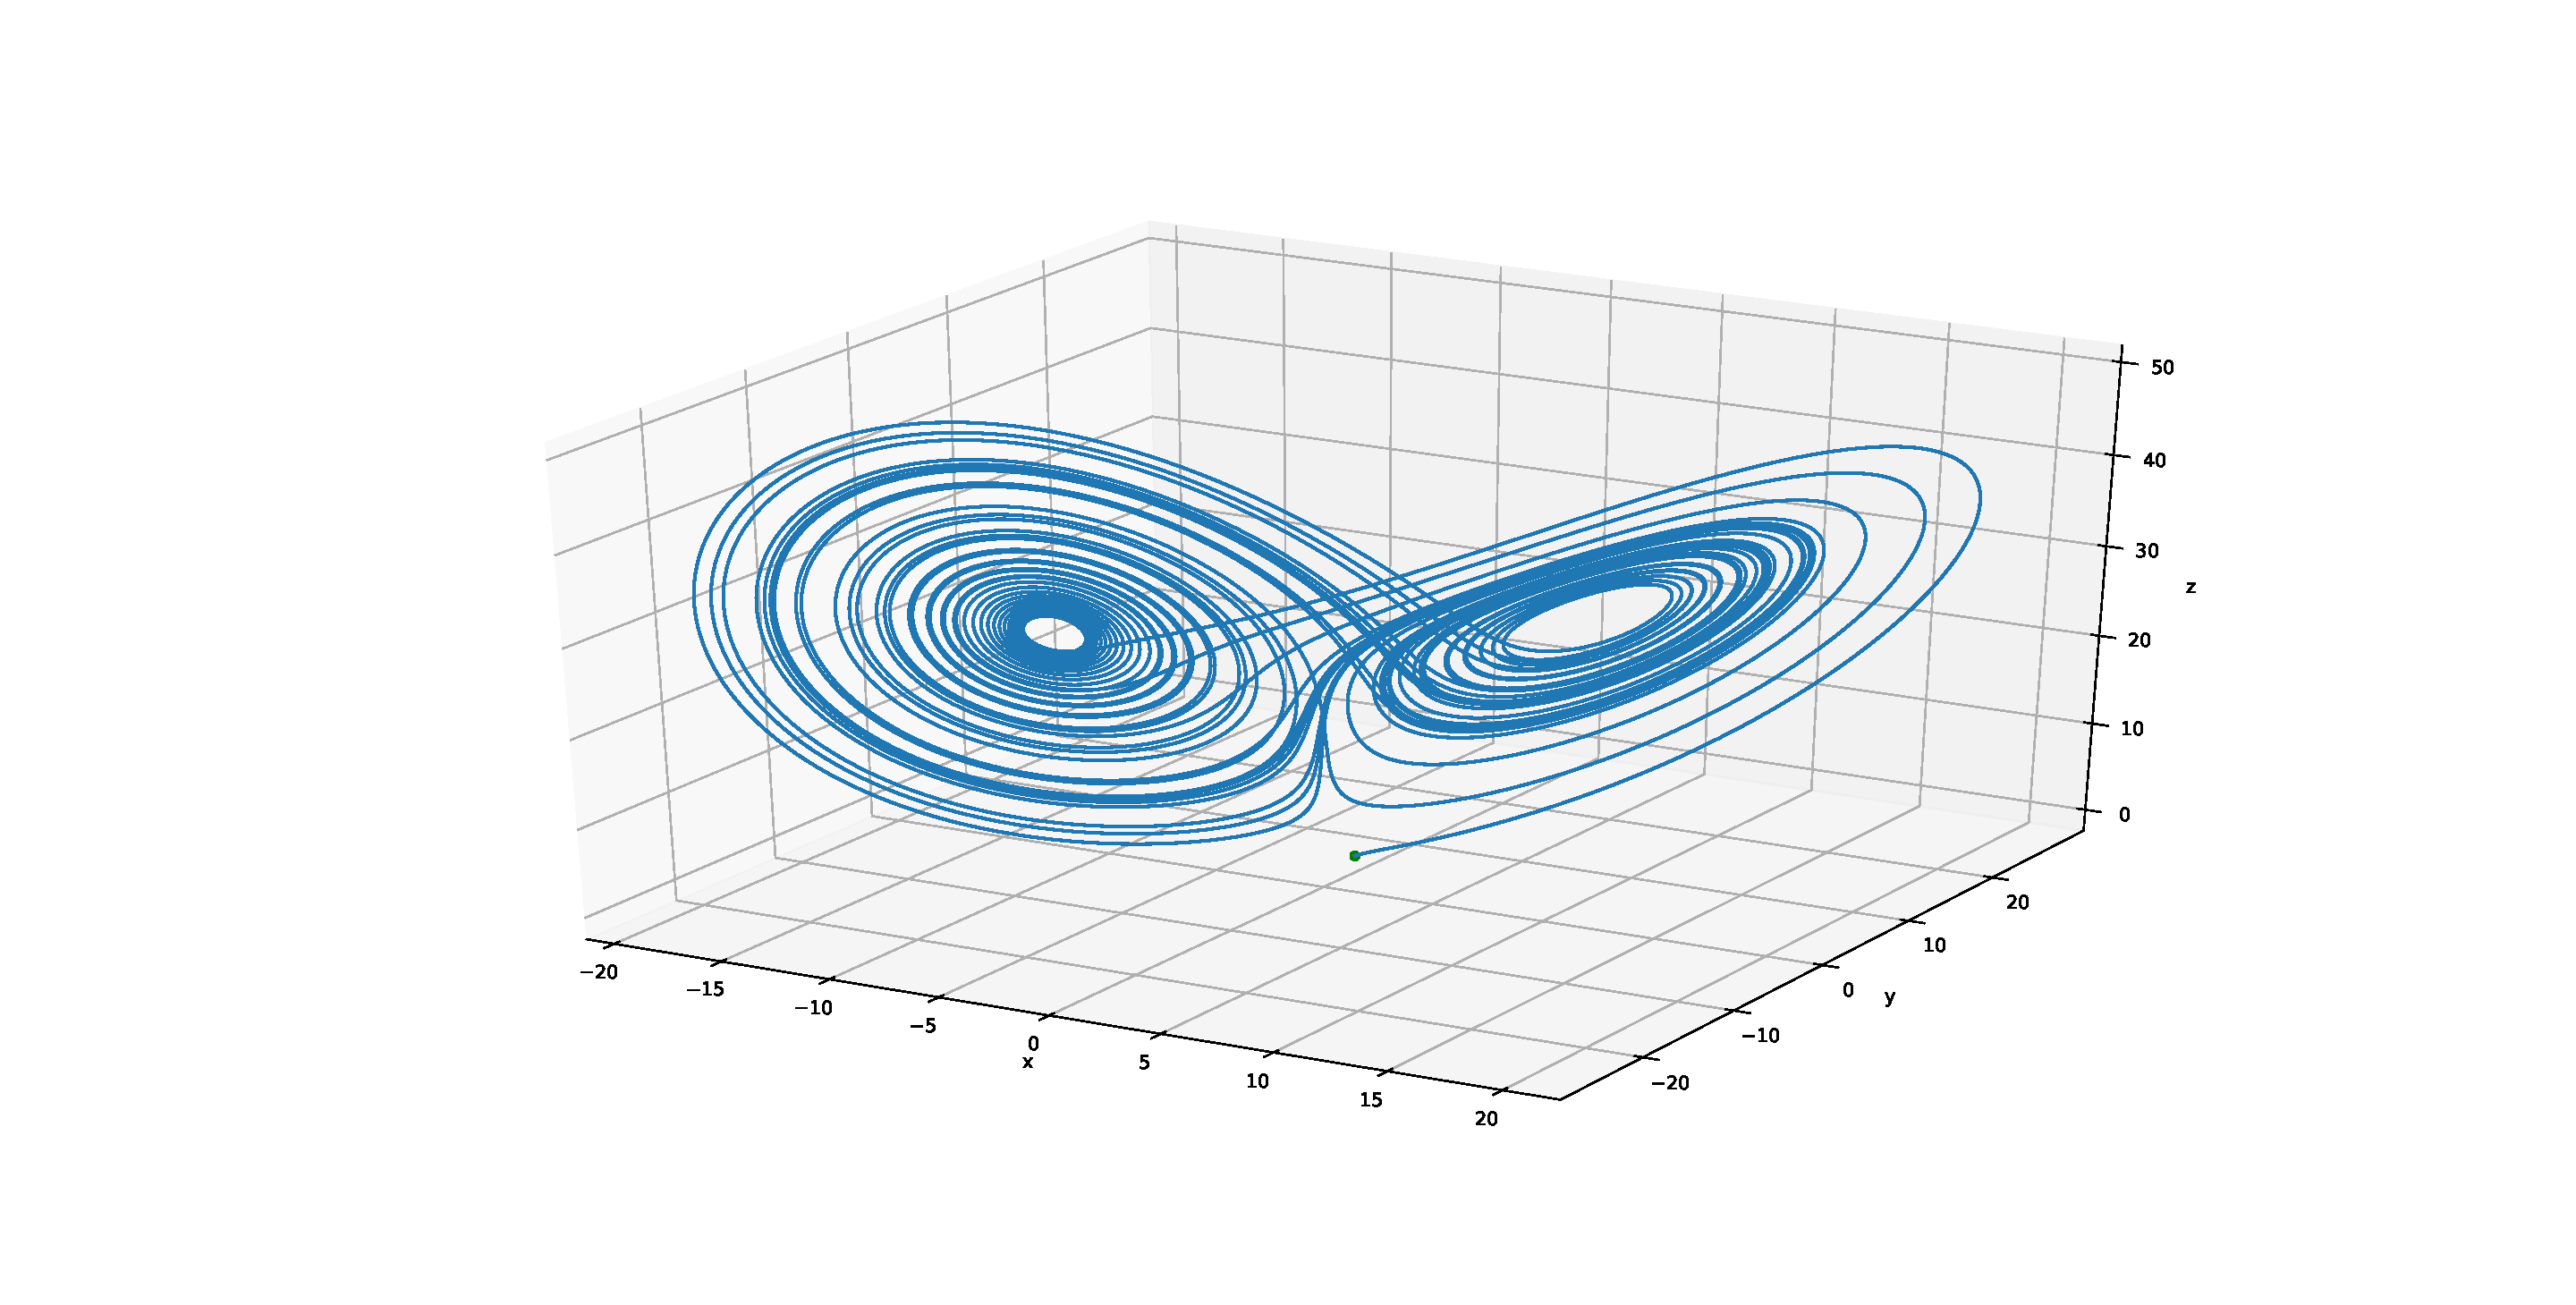
\includegraphics[width=\textwidth]{figures/q2-3d-trajectory}
        \caption{Realization of a 50 seconds simulated trajectory. The initial
        position is indicated by the green dot. The resulting trajectory is chaotic
        (as expected for this set of paramaters).}
        \label{fig:q2-3d-trajectory}
    \end{subfigure}%
    ~
    \begin{subfigure}{0.49\textwidth}
        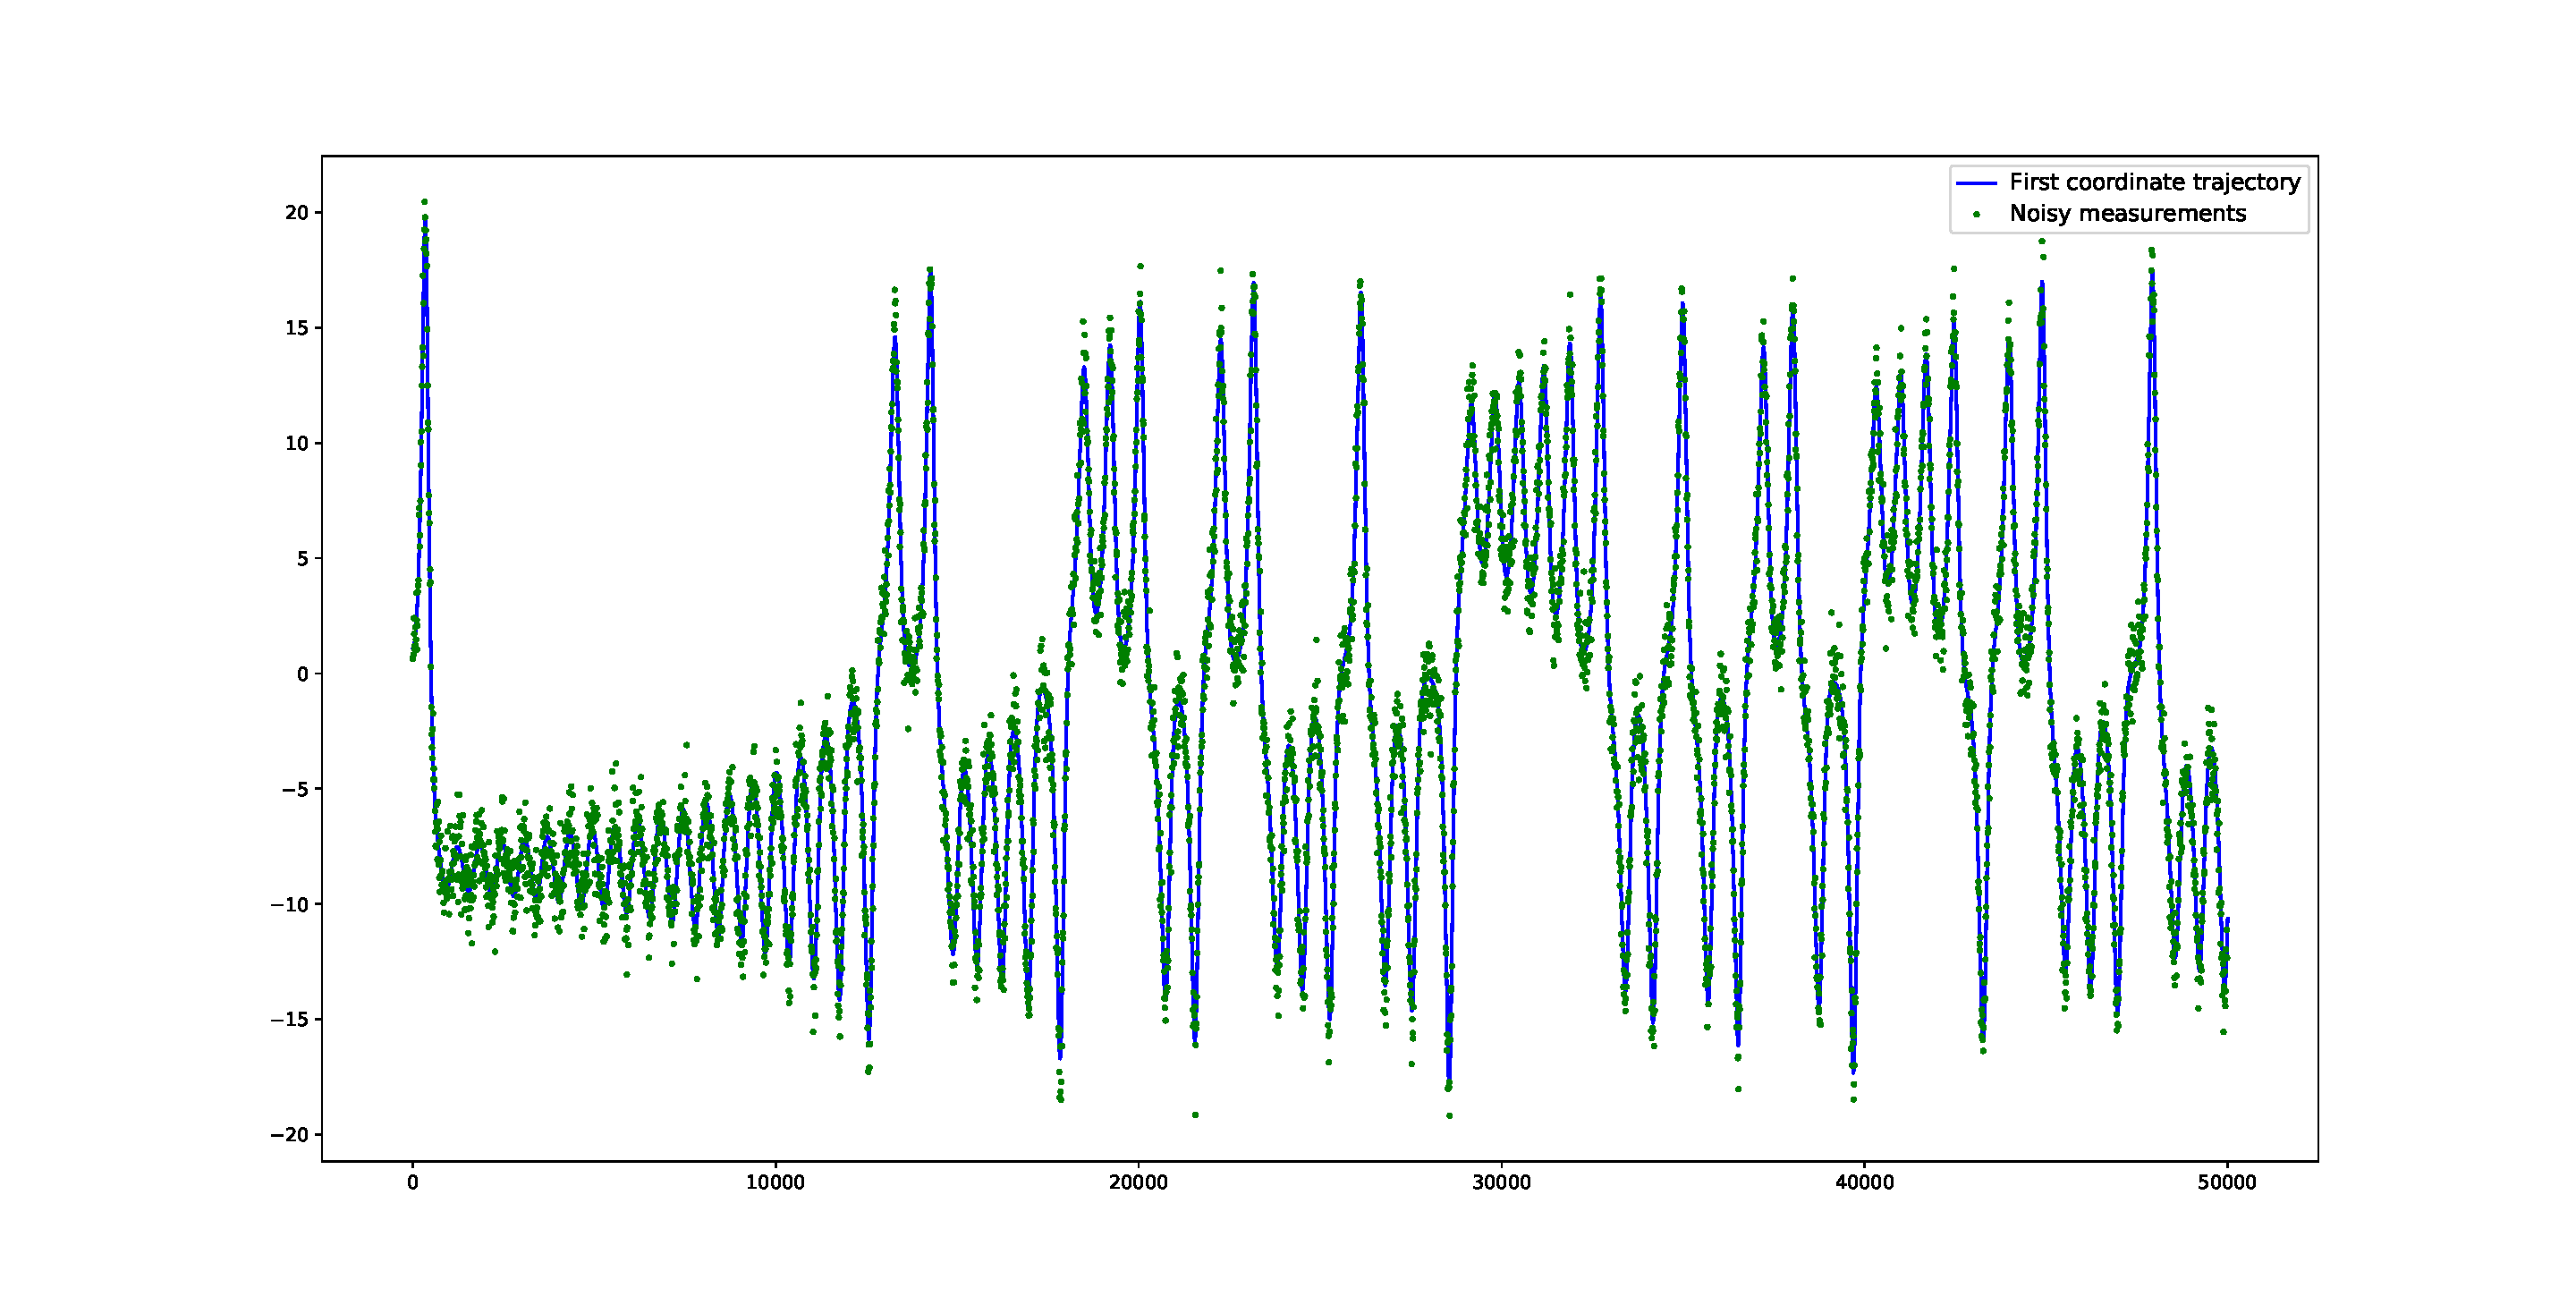
\includegraphics[width=\textwidth]{figures/q2-mes-vs-real}
        \caption{Trajectory of the first coordinates and corresponding noisy
        measurements with $\sigma^2_m = 1$.}
        \label{fig:q2-mes-vs-real}
    \end{subfigure}
    \caption{Simulations and measurements.}
\end{figure}

\FloatBarrier

\section{Sequential Monte Carlo}
\subsection{Observation}

\begin{figure}
    \centering
    \begin{subfigure}{0.49\textwidth}
        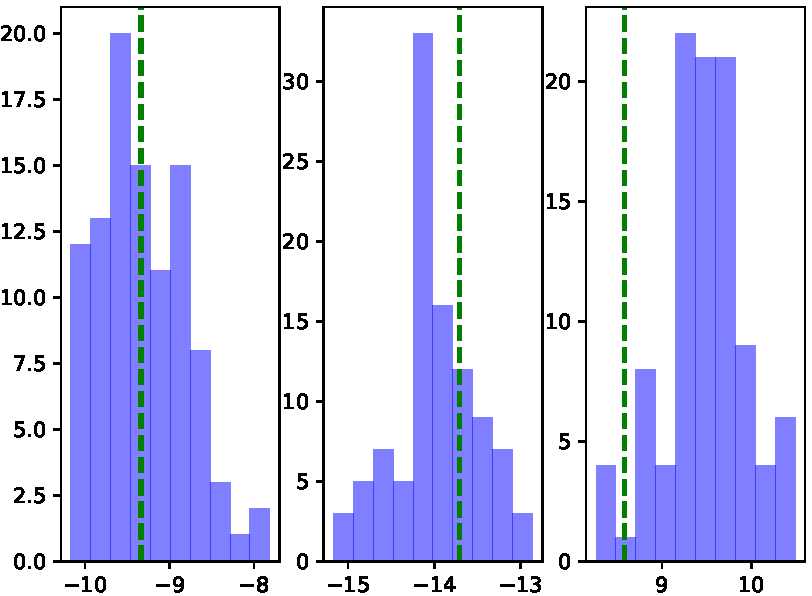
\includegraphics[width=\textwidth]{figures/hist-x-100}
        \caption{Histogram of samples distributions in $x_k$.}
        \label{fig:q3-hist-x-100}
    \end{subfigure}%
    ~
    \begin{subfigure}{0.49\textwidth}
        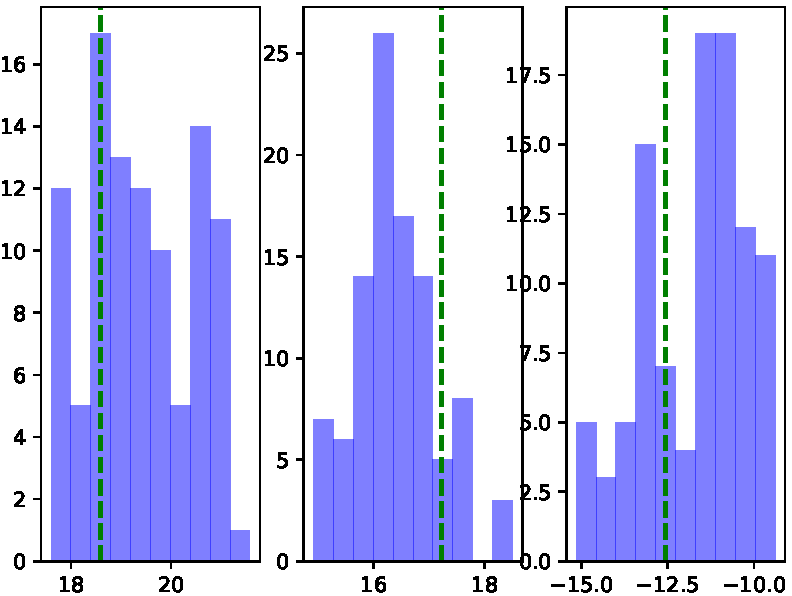
\includegraphics[width=\textwidth]{figures/hist-y-100}
        \caption{Histogram of samples distributions in $y_k$.}
        \label{fig:q3-hist-y-100}
    \end{subfigure}
    \caption{Histogram of samples distributions  at time $t = 0, 5, 15$
    (from left to right) for 100 particles. The dashed green lines represent the real
    values.}
\end{figure}

\begin{figure}
    \centering
    \begin{subfigure}{0.49\textwidth}
        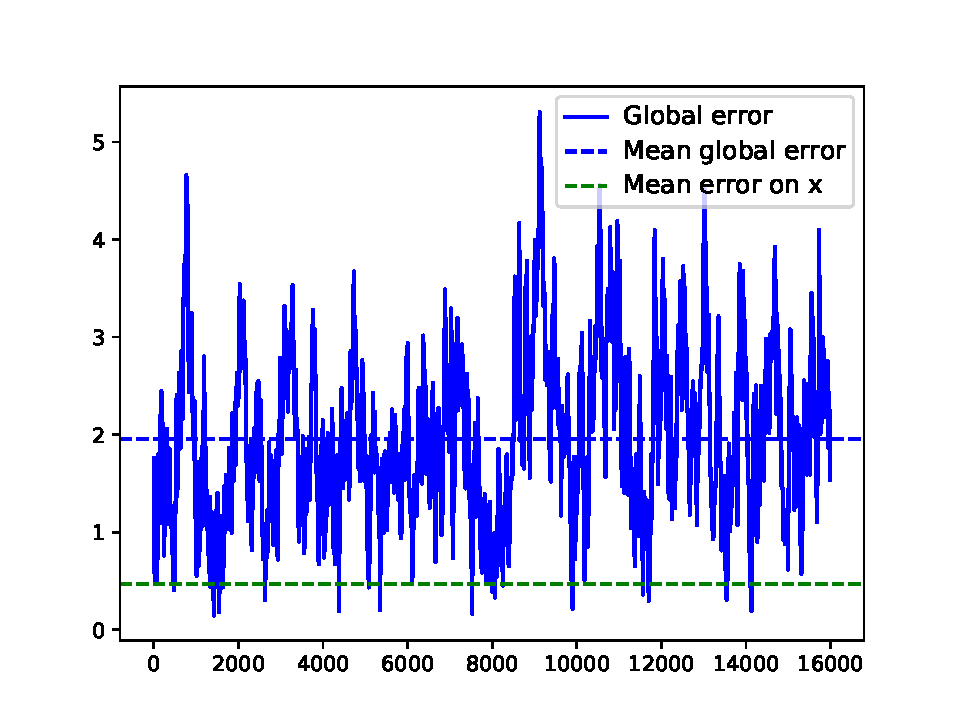
\includegraphics[width=\textwidth]{figures/error-50}
        \caption{For $n=50$ particles.} 
        \label{fig:q3-error-50}
    \end{subfigure}%
    ~
    \begin{subfigure}{0.49\textwidth}
        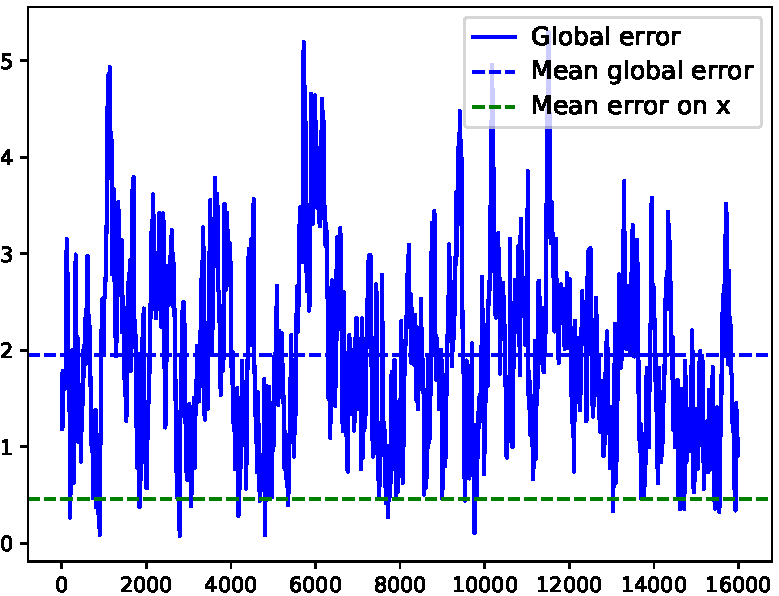
\includegraphics[width=\textwidth]{figures/error-100}
        \caption{For $n=100$ particles.} 
        \label{fig:q3-error-100}
    \end{subfigure}\\
    \begin{subfigure}{0.49\textwidth}
        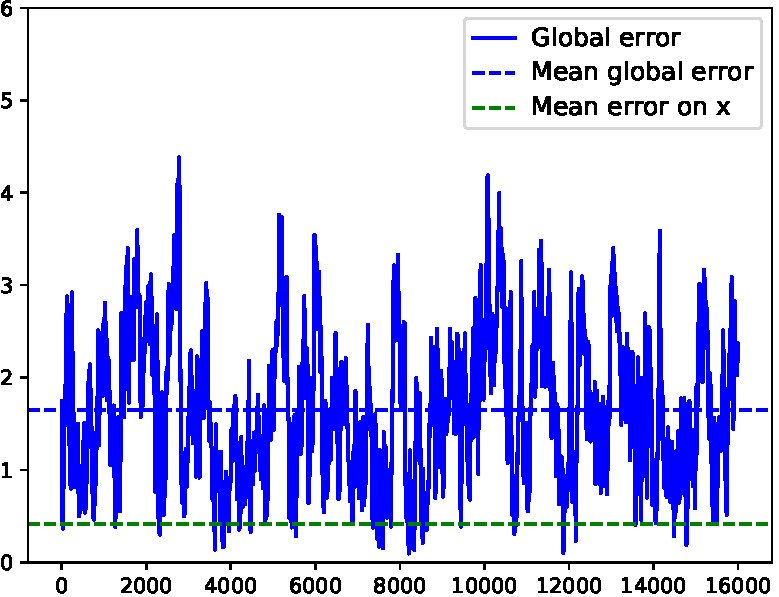
\includegraphics[width=\textwidth]{figures/error-1000}
        \caption{For $n=1000$ particles.} 
        \label{fig:q3-error-1000}
    \end{subfigure}
    \caption{Error as a function of time for different numbers of particles. The blue
    lines correspond to $\norm{\mathbf{x}_t^{\text{real}} - \sum_{i=1}^n
    w_t^i\tilde{\mathbf{x}}_t^i}_2$.
    The mean error on the first coordinate has also been plotted.}
\end{figure}

\begin{figure}
    \centering
    \begin{subfigure}{0.49\textwidth}
        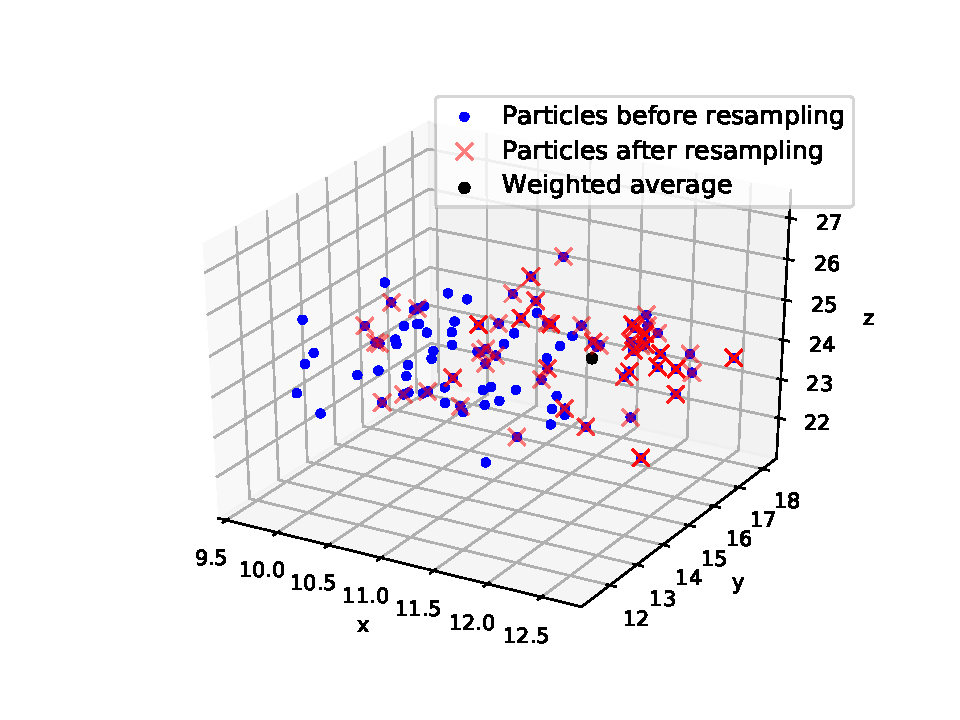
\includegraphics[width=\textwidth]{figures/particles-5-100}
        \caption{At $t=5$.}
        \label{fig:particle-5-100}
    \end{subfigure}%
    ~
    \begin{subfigure}{0.49\textwidth}
        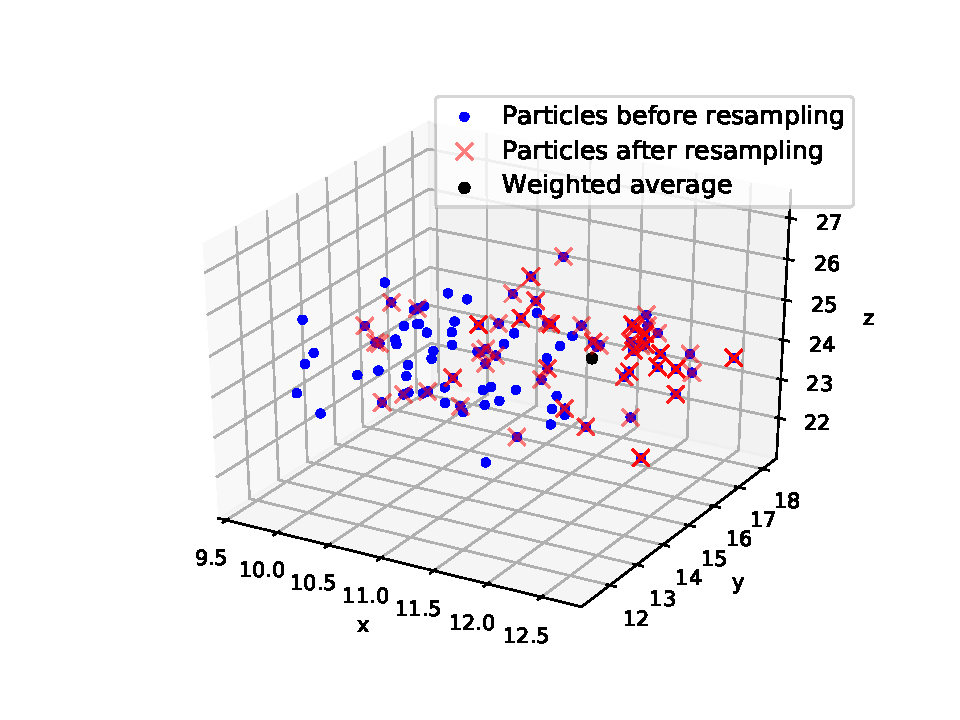
\includegraphics[width=\textwidth]{figures/particles-5-100}
        \caption{At $t=15$.}
        \label{fig:particle-15-100}
    \end{subfigure}
    \caption{Particles before and after resampling for 100 particles.}
\end{figure}

\FloatBarrier

\subsection{Experiments}
\paragraph{Effect of $\sigma^2_0$}
\paragraph{Effect of $\sigma^2_u$}
\paragraph{Effect of $\sigma^2_m$}
\paragraph{Effect of $\delta t$ and $\Delta t$}
\paragraph{Effect of $\Gamma$}

\subsection{Results on the given dataset}


\section{Implementation of an Extended Kalman Filter}

The Extended Kalman Filter amounts to applying a regular Kalman filter to the linearization of the system. Our system can be represented as :


\begin{equation*}
    \begin{cases}
        \vec{x}_{k+1} = F(\vec{x}_k) + \Gamma\vec{u}_k \\
        m_k = x_k + w_k
    \end{cases}.
\end{equation*}

In order to linearize this system, we need to compute the jacobian of $F$, for each time step $k$ :

\begin{equation*}
F_k = 
    \begin{pmatrix}
        1 - a \delta t & a \delta t & 0 \\
        (r - z_k) \delta t & 1 - \delta t & - x_k \delta t \\
        y_k \delta t & x_k \delta t & 1 - b \delta t
    \end{pmatrix}
\end{equation*}

We can then directly apply the Kalman Filter's equations. For prediction :


\[ \vec{\hat{x}}_{k|k-1} = F(\vec{x}_{k-1|k-1}) \]
\[ \vec{P}_{k|k-1} = \vec{F}_{k-1} \vec{P}_{k-1|k-1} \vec{F}_{k-1}^\mathsf{T} + \vec{Q} \]

with $\vec{Q} = \vec{\Gamma} \sigma_u^2$ the covariance matrix of the dynamics' noise.\\
For the update :

\[ \vec{K}_k = \vec{P}_{k|k-1} \vec{H}^\mathsf{T} (\vec{H} ~ \vec{P}_{k|k-1} \vec{H}^\mathsf{T} + R)^{-1} \]

with $R = \sigma_m^2$ and $\vec{H} = 
    \begin{pmatrix}
        1 & 0 & 0 \\
    \end{pmatrix}
$.\\
The updated estimation can then be computed as usual :


\[ \vec{\hat{x}}_{k|k} = \vec{\hat{x}}_{k|k-1} + \vec{K}_k (m_k  - \vec{H} ~ \vec{\hat{x}}_{k|k-1}) \]
\[ \vec{P}_{k|k} = \vec{P}_{k|k-1} - \vec{K}_k ~ \vec{H} ~ \vec{P}_{k|k-1} \]


\end{document}
